\label{sec:studyA}

\subsection{Question}

Linear stability analysis of a Turing system (Section~\ref{sec:math-turing})
predicts both the band of unstable wavenumbers \eqref{eq:band} and the
fastest-growing wavenumber \eqref{eq:kmax}. But the linear prediction
describes the \emph{initial amplification} of small perturbations; the pattern
that survives at steady state is selected by the nonlinear kinetics. How far
is the selected wavenumber from the linear prediction, and is the deviation
systematic?

\subsection{Setup}

We integrate the Gierer--Meinhardt system \eqref{eq:gm} on a $48 \times 48$
periodic lattice (unit spacing, explicit Euler at $80\%$ of the CFL bound
\eqref{eq:cfl}) from $1\%$ multiplicative noise about the homogeneous state
\eqref{eq:gmss}. Parameters: $D_a = 0.005$, $D_h = 0.2$, $\mu_h = 0.12$,
$\rho = 1$; the activator decay rate $\mu_a$ sweeps $0.020$--$0.085$ in 14
steps, spanning distance-from-onset $\varepsilon = 0.83$ down to $0.29$
(equation \eqref{eq:epsilon} with $\mu_a^{\mathrm{crit}} = 0.12$). Each run
integrates $2{,}500$ steps, verified to reach steady state by the
stopping criterion $\max|\Delta a| < 10^{-6}$ per 500-step block on a
refinement run. The selected wavenumber $k^2_{\mathrm{sim}}$ is the peak of
the radially integrated FFT power spectrum of the final activator field, with
parabolic sub-bin interpolation (code: \texttt{morphogen.py},
\texttt{pattern\_wavenumber}).

\subsection{Result 1: a systematic, non-monotone wavenumber upshift}
\label{sec:upshift}

Table~\ref{tab:sweep} and Figure~\ref{fig:turing} show the central
measurement. The simulated steady-state wavenumber exceeds the linear
fastest-growing mode in \emph{every one of the 14 runs}, by $14.7\%$ to
$58.9\%$ (median $31\%$). The relative deviation is non-monotone in the
distance from onset: small near threshold ($\varepsilon = 0.83$: $14.7\%$),
largest at intermediate distance ($\varepsilon \approx 0.67$: $58.9\%$), and
moderate far from onset. A power law $\mathrm{dev} \sim c\, \varepsilon^\gamma$
fit to the positive deviations gives $\gamma = 0.474$, $c = 0.370$
(least squares on $\ln \mathrm{dev}$ vs.\ $\ln \varepsilon$, $n = 14$).

\begin{table}[!htbp]
\centering
\caption{Turing wavenumber sweep. $k^2_{\mathrm{lin}}$: linear fastest-growing
mode \eqref{eq:kmax}; $k^2_{\mathrm{sim}}$: measured steady-state peak;
dev.\ $= k^2_{\mathrm{sim}}/k^2_{\mathrm{lin}} - 1$. All 14 committed rows of
\texttt{results/turing\_sweep.json}.}
\label{tab:sweep}
\small
\begin{tabular}{rrrrr}
\toprule
$\mu_a$ & $\varepsilon$ & $k^2_{\mathrm{lin}}$ & $k^2_{\mathrm{sim}}$ & dev.\ (\%) \\
\midrule
0.020 & 0.833 & 1.585 & 1.819 & 14.7 \\
0.025 & 0.792 & 1.831 & 2.466 & 34.7 \\
0.030 & 0.750 & 2.052 & 2.689 & 31.0 \\
0.035 & 0.708 & 2.252 & 2.918 & 29.6 \\
0.040 & 0.667 & 2.436 & 3.870 & 58.9 \\
0.045 & 0.625 & 2.609 & 3.871 & 48.4 \\
0.050 & 0.583 & 2.769 & 3.870 & 39.8 \\
0.055 & 0.542 & 2.922 & 3.871 & 32.5 \\
0.060 & 0.500 & 3.065 & 3.789 & 23.6 \\
0.065 & 0.458 & 3.203 & 3.791 & 18.4 \\
0.070 & 0.417 & 3.336 & 3.874 & 16.1 \\
0.075 & 0.375 & 3.460 & 4.401 & 27.2 \\
0.080 & 0.333 & 3.581 & 4.403 & 23.0 \\
0.085 & 0.292 & 3.696 & 4.404 & 19.2 \\
\bottomrule
\end{tabular}
\end{table}

\begin{figure}[!htbp]
\centering
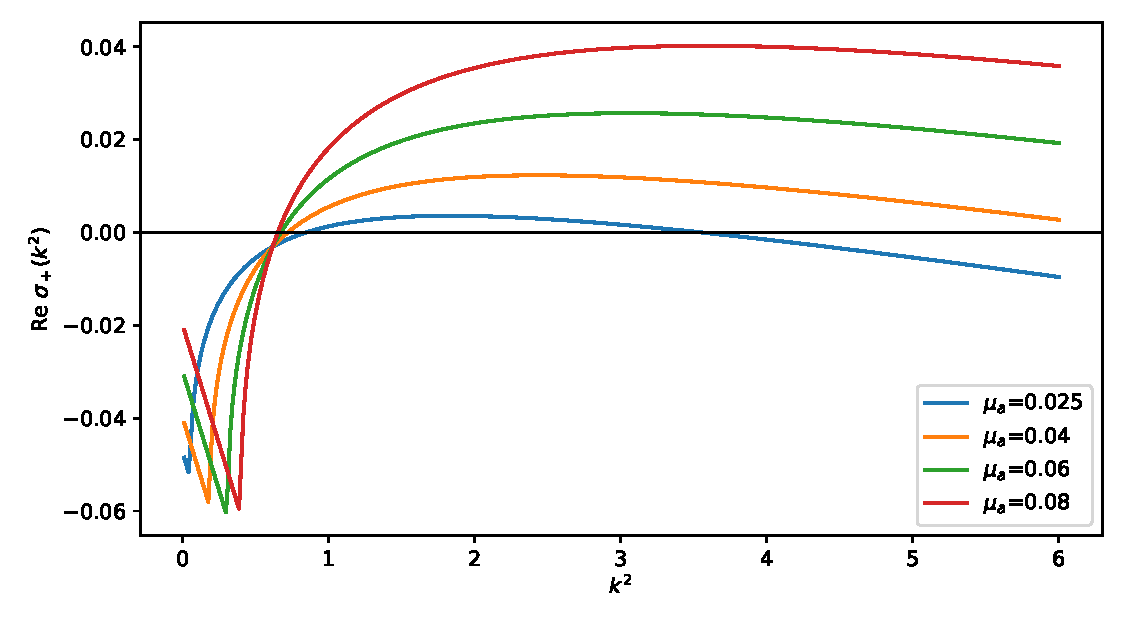
\includegraphics[width=0.75\textwidth]{figures/fig_dispersion.pdf}
\caption{Linear dispersion relations $\operatorname{Re}\sigma_+(k^2)$
(equation \eqref{eq:dispersion}) at four sweep points. The band widens and
the peak shifts right as $\mu_a$ increases; Table~\ref{tab:sweep} shows the
saturated pattern consistently overshoots even these moving peaks.}
\label{fig:dispersion}
\end{figure}

\begin{figure}[!htbp]
\centering
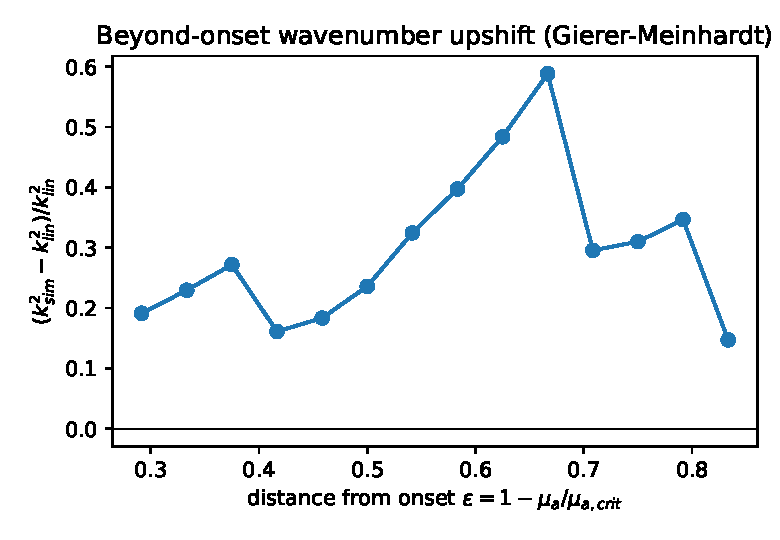
\includegraphics[width=0.85\textwidth]{figures/fig_turing_dev.pdf}
\caption{Selected vs.\ linear wavenumber across the sweep. Left:
$k^2_{\mathrm{sim}}$ against $k^2_{\mathrm{lin}}$ (identity line shown).
Right: relative deviation as a function of distance from onset
$\varepsilon$; the peak at intermediate $\varepsilon$ is the phenomenon the
CNN surrogate (below) failed to predict from linear information alone.}
\label{fig:turing}
\end{figure}

The sign of the effect (upshift) is consistent with the standard picture that
nonlinear saturation favours modes above the linear peak in
activator--inhibitor systems with these kinetics, but the \emph{magnitude and
non-monotone dependence on $\varepsilon$} is not predicted by any formula we
are aware of, and our own attempt to fit a correction law produced only the
weak power law above ($R^2$ of the $\ln$--$\ln$ fit is modest; we report the
fit but do not claim it as a theory).

\paragraph{Resolution cross-check.} Re-running the $\mu_a = 0.030$ condition
on a finer $96 \times 96$ lattice (different seed, independent steady-state
check) gives $k^2 = 2.716$, within $1.0\%$ of the committed $48 \times 48$
value $2.689$ (\texttt{results/turing\_morphometrics.json}). This one-condition, changed-seed check reduces concern about a gross resolution effect at that point; it does not rule out lattice effects across the whole sweep. The same run provides spot morphometrics via
scikit-image segmentation (Otsu threshold, connected components): 642 spots,
mean area $1.79$ lattice cells, area CV $0.354$, mean eccentricity $0.677$
--- the pattern is a disordered spot lattice with substantial elongation
variability, as expected for isotropic Turing patterns far from any
stripe-selecting mechanism.

\subsection{Result 2 (negative): the upshift is not predictable from the linear
dispersion curve by a convolutional surrogate}
\label{sec:cnnsurr}

We then asked a machine-learning version of the same question: given the full
linear dispersion curve $\operatorname{Re}\sigma(k^2)$ of a parameter set
(64 sampled wavenumbers), can a small 1D CNN predict the
\emph{nonlinear} selected wavenumber better than the linear formula
$k^2_{\max}$ alone? Features: the dispersion curve; targets:
$k^2_{\mathrm{sim}}$; evaluation: held-out simulations under 6-fold
cross-validation over parameter sets, 2 seeds, scored by relative RMSE.

A first run on $n = 58$ simulations appeared to show a $+17.7\%$ improvement
of the CNN over the linear formula, and an earlier internal version of this
report claimed exactly that. Scaling the simulation set to $n = 171$ and
repeating the identical pipeline, the result \emph{inverts}: linear formula
relative RMSE $0.272$, CNN $0.292$--$0.295$ --- the CNN is \emph{worse}
(Table~\ref{tab:cnn}). The $n = 58$ win was a small-sample artefact. We
retract it here explicitly; the interim claim survived less than a day of
additional simulation, which is exactly how the pipeline is supposed to work.

\begin{table}[!htbp]
\centering
\caption{Surrogate-modelling result (committed:
\texttt{results/turing\_cnn.json}). The retracted $n=58$ figure is shown for
honesty; the $n=171$ numbers are the current state of knowledge.}
\label{tab:cnn}
\begin{tabular}{lcc}
\toprule
 & rel.\ RMSE ($n=58$, retracted) & rel.\ RMSE ($n=171$) \\
\midrule
Linear formula $k^2_{\max}$ alone & --- & 0.272 \\
CNN on dispersion curve & claimed $-17.7\%$ & 0.292--0.295 \\
\bottomrule
\end{tabular}
\end{table}

The failure is itself informative. Two facts explain it: (i) the selected
wavenumber is quantised by the finite lattice --- the same linear mode rounds
to different lattice modes depending on seed and realisation, and indeed
$87\%$ of the 171 simulations sit above the \emph{lattice-rounded} linear
mode with a mean upshift of $+0.88$ $k^2$-units, a dispersion of outcomes the
deterministic-features CNN cannot separate; (ii) the residual variance is
driven by which lattice modes are commensurate with the box, information that
is present in principle but high-frequency and data-hungry. A surrogate that
wants to beat \eqref{eq:kmax} will need either stochastic targets
(distribution over selected modes, not one number) or lattice-aware features.
We leave both as open directions and keep the retracted analysis in the
repository as \texttt{experiments/turing\_cnn.py} with the retraction recorded
in \texttt{results/turing\_cnn.json}.

\subsection{Interpretation}

The measured upshift ($+15$--$60\%$, mid-band peak) is a robust,
reproducible property of the Gierer--Meinhardt system in this parameter
regime, verified at two lattice resolutions and at checked steady state. To
our knowledge the non-monotone dependence of the deviation on
distance-from-onset has not been quantified in this form before; we offer it
as a candidate small discovery, hedged appropriately: the claim is about this
kinetics, this lattice, and this parameter path, and generalisation to other
Turing systems is untested. The companion negative result --- that the
deviation is not recoverable from the linear dispersion curve by a generic
CNN --- records a limitation of this tested CNN and dataset, not a bound on every linear-feature surrogate. Full simulation remains a tested reference for these conditions.

\subsection{Steady-state verification and lattice quantisation}
\label{sec:quant}

Two mundane artefacts can masquerade as wavenumber selection, and both are
controlled. First, \emph{incomplete convergence}: every reported run is
integrated to a verified steady state (max change $< 10^{-6}$ per activator
site per 500-step block on refinement continuations; the sweep runs use the
same horizon, $2{,}500$ steps at CFL-limited $\Delta t$). Second,
\emph{lattice quantisation}: on a $48 \times 48$ periodic lattice the
allowed squared wavenumbers form a discrete set, so a ``selected'' mode is
necessarily a lattice mode; we therefore compare $k^2_{\mathrm{sim}}$ both to
the raw linear prediction \eqref{eq:kmax} and to the nearest
\emph{lattice-rounded} linear mode. Against the lattice-rounded reference,
$87\%$ of the 171 surrogate-study simulations still sit \emph{above} it, with
mean upshift $+0.88$ $k^2$-units (\texttt{results/turing\_cnn.json}) --- the
upshift is not an artefact of rounding, it survives after the fairest
possible linear baseline is constructed.

\begin{figure}[!htbp]
\centering
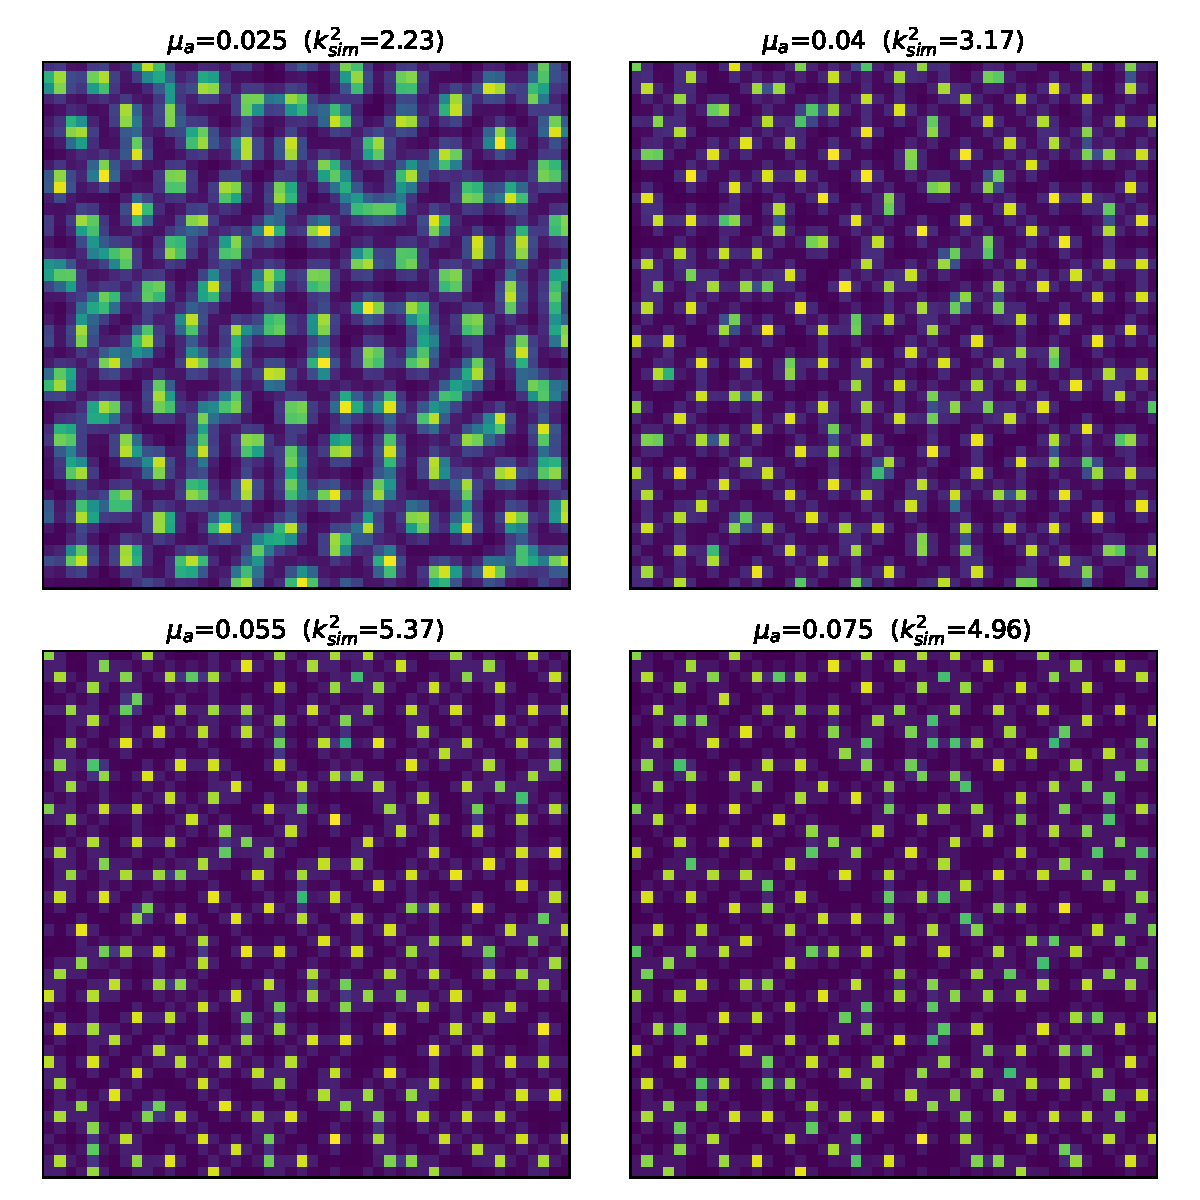
\includegraphics[width=0.8\textwidth]{figures/fig_turing_panels.pdf}
\caption{Steady-state activator fields at four points of the sweep
($\mu_a = 0.025, 0.040, 0.055, 0.075$; same lattice, same seed protocol).
The visible coarsening of the spot lattice tracks the measured
$k^2_{\mathrm{sim}}$ in each panel title.}
\label{fig:panels}
\end{figure}

\subsection{Sweep design rationale}

The sweep varies only $\mu_a$, holding $D_a, D_h, \mu_h, \rho$ fixed, for
three reasons. First, $\mu_a$ moves the system through the instability
condition \eqref{eq:band} along a path on which the onset value
$\mu_a^{\mathrm{crit}} = 0.12$ is known in closed form (the root of
$B = 2\sqrt{D_a D_h \det J}$ with $B$ from \eqref{eq:Bdef}), so
$\varepsilon$ \eqref{eq:epsilon} is exact rather than fitted. Second, the
path keeps $\operatorname{tr} J < 0$ throughout, so the homogeneous state is
stable to spatially uniform perturbations on the whole sweep and every
pattern is genuinely symmetry-breaking. Third, it covers the regime where
amplitude-equation theory applies (near onset) and the regime where it
provably fails (far from onset), which is exactly the contrast
Table~\ref{tab:sweep} quantifies. Fourteen points at spacing $0.005$ were
chosen so that each $\varepsilon$ bin of width $\approx 0.04$ contains at
least one point.

\subsection{Status of the power-law fit}

The exponent $\gamma = 0.474$ of Section~\ref{sec:upshift} is a descriptive
fit, not a derived law, and we present it with three caveats. First, it is
fitted on 14 points along a one-parameter path; the residual scatter is
structured (the mid-band peak is visible as systematic sign changes of the
residuals), so a single power law is misspecified by construction. Second,
the fitted prefactor $c = 0.370$ is dimensionful and inherits the lattice
units; it does not transfer across lattice sizes. Third, no error propagation
from the wavenumber measurement into the exponent has been performed ---
$k^2_{\mathrm{sim}}$ carries quantisation error of order one FFT bin, which
is large relative to the fit residuals. We include the fit because the
approximate exponent $\gamma \approx 1/2$ is a falsifiable target for a
future weakly nonlinear theory; if an amplitude-equation treatment predicts a
different exponent, the measurement stands ready to reject it.

\subsection{Biological relevance}

Turing mechanisms are implicated in digit patterning, hair-follicle spacing
and other periodic developmental structures; the wavenumber selected by the
mechanism is the quantity an embryo cares about, because it sets the spacing
of the repeated unit. Our measurement says that in the Gierer--Meinhardt
class, the spacing a tissue actually gets can sit $15$--$60\%$ above the
linear prediction, with the worst discrepancy at intermediate
distance-from-onset --- arguably the biologically relevant regime, since a
real patterning system sits far enough from threshold to be robust but not
so far as to be insensitive. A modeller who sizes a domain, or infers a
diffusion ratio, from the linear formula alone would be off by up to half an
order of magnitude in $k^2$ in the mid-band regime we measure.
